\section{Programmiersprachen}
\setauthor{Felix Dumfarth}

\subsection{Java}

\begin{figure}[hbt!]
    \centering
    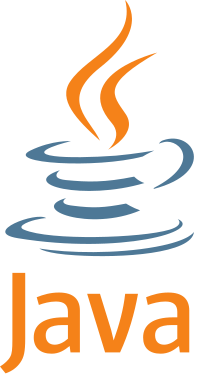
\includegraphics[scale=0.5]{pics/java}
    \caption{Java Logo\cite{java}}
    \label{fig:impl:java}
\end{figure}

Für das Backend haben wir uns für Java entschieden.
Java ist laut dem TIOBE-Index\cite{tiobe} eine der populärsten Programmiersprachen.
Java ist eine objektorientierte Programmiersprache und besitzt dadurch Klassen und Vererbung\cite{java}.

\subsection{Python}
Phyton ist eine Programmiersprache die mehrere Arten der Programmierung unterstützt wie zum Beispiel die objektorientierte, die aspektorientierte und die funktionale Programmierung.
Phyton wird oft für Machine Learning verwendet, auch bei uns kommt Phyton bei Rasa zum einsatz.
Zum einen ist Rasa ein Python framework zum anderen werden die Custom-Actions mit Phyton umgesetzt.

\subsection{Typescript}
Typescript ist eine Programmiersprache die eine kompakte und einfache Syntax zur Programmierung von Webseiten und Anwendungen bietet.
Typescript baut auf Javascript auf und hilft zum Beispiel beim frühzeitigen Erkennen von Fehlern.

\section{Technologien}
\setauthor{Felix Dumfarth}

\subsection{REST Service}
REST steht für Representational State Transfer.
REST Anfragen sind CRUD – Operationen (Create, Read, Update, Delete).
Diese sind GET, POST, PUT und DELETE Requests.
Außerdem gibt es noch OPTIONS, PATCH, HEAD, TRACE
und CONNECT diese werden aber in der vorliegenden Arbeit nicht benutzt.

* Die GET Methode ist zum Abfragen da, es soll ein Request geschickt werden und nur Daten zurückgeben werden, es soll jedoch auf dem Server wohin die Anfrage geschickt worden ist nichts geschehen außer Daten lesen.

* Bei POST sollen Daten hinzugefügt werden, im Standardfall ist in der Respone der URI der neu gespeicherten Daten

* Bei PUT sollen Daten hinzugefügt werden, falls diese schon existieren werden Sie upgedatet und falls nicht, wird ein neuer Eintrag erstellt.

* Bei DELETE sollen Daten gelöscht werden.

\subsection{Quarkus}\label{quarkus}
Quarkus ist ein Framework für Java welches sich auf die REST-Service-API ausrichtet. Wir haben unser Backend\ref{sec:backend} mit Quarkus umgesetzt.

\subsection{Angular}
Angular ist ein auf TypeScript basierendes Framework für Webseiten.
Gedacht ist es für Single Page Applications.
Unser Chat Widget\ref{sec:chat-widget} und unser Dashboard\ref{sec:dashboard} wurden mit Angular umgesetzt



\section{Werkzeuge}
\setauthor{Felix Dumfarth}

\subsection{Rasa X}\label{subsec:rasa-x}
Rasa X ist ein Werkzeug um Conversation-Driven Development\ref{cdd} in die Tat umzusetzen\cite{rasax}.
Rasa X liegt über Rasa und liefert dadurch erweiterte Funktionalitäten, die man nur mit Rasa nicht hätte.
Wir haben Rasa X mit Docker Compose\cite{rasaxDocker} auf unserer VM installiert\ref{sec:systemarchitektur}.

Rasa X kommt mit einer grafischen Weboberfläche, auf dieser kann man sich seine Intents, Responses und so weiter verändern und ansehen.
Man kann auch sein Model trainieren oder ein Model hochladen.

Wir benutzen jedoch unser eigenes Dashboard und benötigen die grafische Oberfläche nicht sondern nur die erweiterte Funktionalität die auch über die API aufgerufen werden kann.

Damit unser Frontend auf Rasa, welches eine Ebene unter Rasa X liegt, zugreifen kann, muss das automatisch erstellte credentials.yml file bearbeitet werden:

\begin{lstlisting}[language=yml]
rasa:
url: ${RASA_X_HOST}/api
rest:
\end{lstlisting}

\subsection{IntelliJ IDEA}
IntelliJ ist ein IDE welche eine Vielzahl von Programmiersprachen unterstützt und hauptsächlich für diese Arbeit verwendet wird.

\subsection{GitHub}
GitHub ist ein online Git Repository welches die gemeinsame Programmierung von Programmierern und Entwicklern erleichtert.

\subsection{Docker}
Docker ist einer der bekanntesten Container-Manager.
